\documentclass[11pt,a4paper]{article}
\usepackage[utf8]{inputenc}
\usepackage[T1]{fontenc}
\usepackage[brazil]{babel}
\usepackage[top=2.5cm,bottom=2cm,left=2.5cm,right=2cm]{geometry}
\usepackage{booktabs}
\usepackage{enumitem}
\usepackage{graphicx}
\usepackage{tcolorbox}
\usepackage{hyperref}

\title{\textbf{Relatório de Acompanhamento Diário -- Experiência Criativa}\\
\large Estudo de Caso: Arquitetura Segura para Rede de Farmácias (PUCPR)}
\author{\textbf{Equipe:} Gustavo Kawano, Henrique Papai, Edson Renato}
\date{Setembro de 2026}

\begin{document}

\maketitle

\section{Identificação da Equipe}
\textbf{Integrantes participantes:} Gustavo Kawano, Henrique Papai e Edson Renato.

\section{Configuração Obrigatória de Usuários (Menor Privilégio)}
Conforme exigência do projeto acadêmico, os usuários padrão foram configurados no ambiente com privilégios estritamente mínimos (\textit{least privilege}):
\begin{itemize}[noitemsep]
    \item \textbf{Usuário de Sistema (OS / Banco de Dados / Container):} \texttt{teste} | \textbf{Senha:} \texttt{T35t3} \\
    \textit{Privilégio:} Role no PostgreSQL com acesso apenas de leitura (\texttt{SELECT}) nas tabelas públicas e na view anonimizada; usuário não-root no container Linux.
    \item \textbf{Usuário para Aplicações (Keycloak IAM / Portal Web):} \texttt{teste@pucparana.com} | \textbf{Senha:} \texttt{Teste@2026} \\
    \textit{Privilégio:} Papel restrito de \texttt{cliente} no Keycloak, sem acessos administrativos ou de farmacêutico.
\end{itemize}

\section{Backlog do Projeto}
\begin{itemize}[noitemsep]
    \item Segmentação de redes Docker (DMZ 172.20.0.0/24 e Interna 172.21.0.0/24).
    \item WAF ModSecurity com OWASP CRS e regras DLP contra vazamento de CPF e cartões.
    \item IDS/IPS Suricata com 11 regras alinhadas às táticas do MITRE ATT\&CK.
    \item Aplicação e-commerce (Flask), PostgreSQL com view LGPD e Keycloak (MFA).
    \item SIEM Wazuh completo (Manager, Indexer OpenSearch, Dashboard e Agentes).
    \item Pipeline de anonimização LGPD com $k$-anonimato ($k \ge 1$).
    \item Migração para 2 VMs Linux com pfSense e automação dos 4 cenários de teste.
\end{itemize}

\section{Atividades Realizadas}
\begin{itemize}[noitemsep]
    \item \textbf{Infraestrutura:} Implementação das composições \texttt{docker-compose.dmz.yml} e \texttt{docker-compose.internal.yml} com 10 containers integrados e operacionais.
    \item \textbf{Defesa de Borda:} ModSecurity ativo na porta 80 bloqueando SQL Injection (\texttt{403}) e ferramentas maliciosas; regras DLP ativas contra exposição de CPF.
    \item \textbf{Detecção:} Suricata monitorando tráfego lateral e exfiltração em tempo real.
    \item \textbf{Identidade e Banco:} Keycloak com realm e MFA importados; PostgreSQL estruturado com dados sintéticos e view anonimizada.
    \item \textbf{SIEM:} Cluster Wazuh Indexer inicializado (\texttt{GREEN}), Dashboard ativo na porta 5601 e agentes DMZ/Interno registrados.
\end{itemize}

\section{Atividades em Desenvolvimento}
\begin{itemize}[noitemsep]
    \item Transferência dos serviços para as duas VMs Linux dedicadas integradas com o firewall pfSense de laboratório.
    \item Ajuste da interface de rede de captura do Suricata na VM Linux.
    \item Elaboração dos scripts executáveis (\texttt{.sh}) para demonstrar os 4 cenários do relatório.
\end{itemize}

\section{Principais Dificuldades}
\begin{itemize}[noitemsep]
    \item \textbf{Permissões em Volumes Somente Leitura (\texttt{:ro}):} Incompatibilidade de escrita em scripts de inicialização do NGINX/Suricata, resolvida injetando as regras no diretório pós-CRS.
    \item \textbf{Hardening no Docker Desktop:} Diretiva \texttt{cap\_drop: ALL} impedia a inicialização do PostgreSQL e Wazuh Agent; solucionada com privilégios mínimos operacionais e isolamento de rede.
    \item \textbf{Inicialização do OpenSearch:} O Wazuh Indexer subiu desconfigurado; resolvido executando a rotina do \texttt{securityadmin.sh} com certificados TLS internos.
\end{itemize}

\newpage

\section{Evidências de Execução -- Screenshots dos Momentos Críticos}

Abaixo constam as capturas de tela dos 3 momentos críticos desenvolvidos, com correlação explícita às atividades do quadro no Trello:

\subsection{Momento 1: Teste Funcional do Web Server e Banco de Dados}
\textbf{Atividade Trello correspondente:} \textit{Segmentação de Redes Docker / PostgreSQL + View Anonimizada LGPD} (Coluna: Concluído).

\begin{figure}[h!]
    \centering
    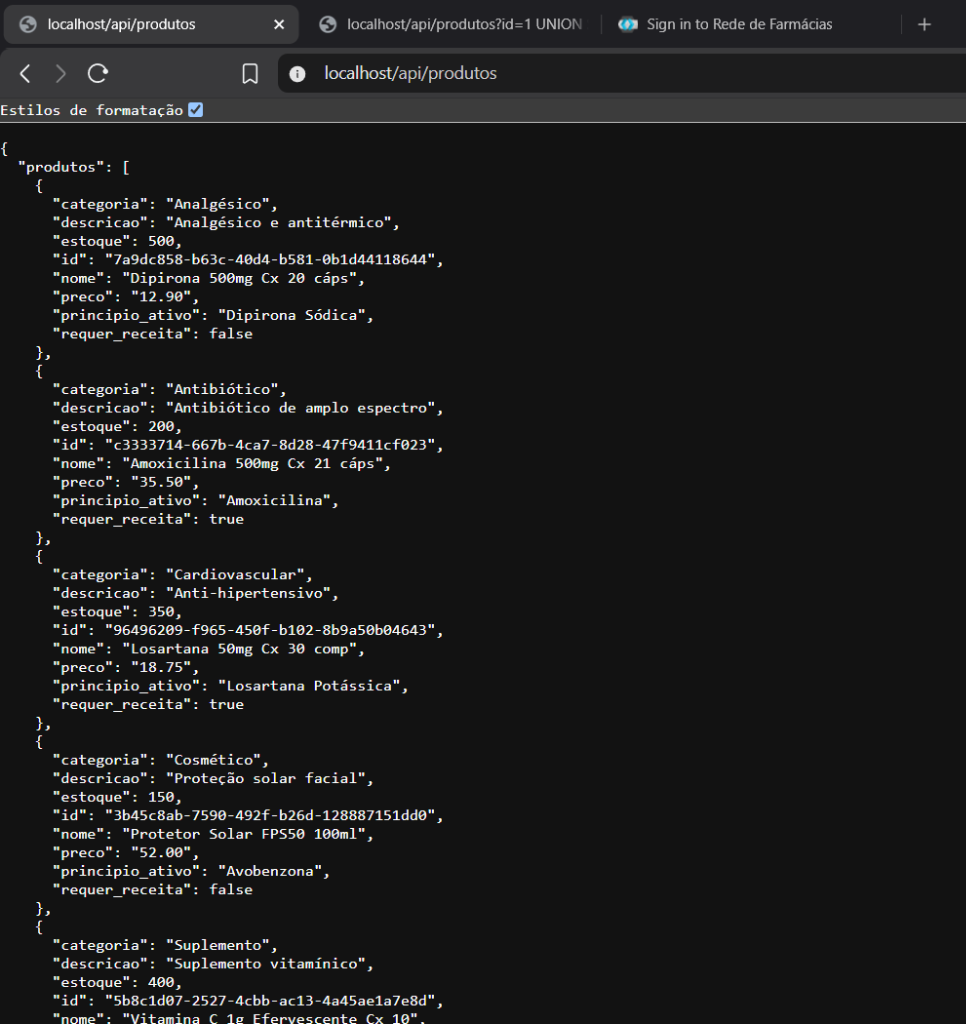
\includegraphics[width=0.82\textwidth]{images/print1_webserver_produtos.png}
    \caption{Resposta da API \texttt{/api/produtos} consumindo dados do PostgreSQL através do WAF na porta 80.}
    \label{fig:momento1}
\end{figure}

\textbf{Descrição do que está sendo feito:} Validação funcional da comunicação entre a DMZ e a Rede Interna. O Web Server de e-commerce recebe a requisição no endpoint \texttt{http://localhost/api/produtos} através do proxy reverso NGINX/WAF e retorna em formato JSON o catálogo de medicamentos consultado no PostgreSQL com usuário de menor privilégio.

\vspace{0.4cm}

\subsection{Momento 2: Teste de Segurança da Camada Perimetral (WAF ModSecurity)}
\textbf{Atividade Trello correspondente:} \textit{WAF ModSecurity + OWASP CRS + DLP} (Coluna: Concluído).

\begin{figure}[h!]
    \centering
    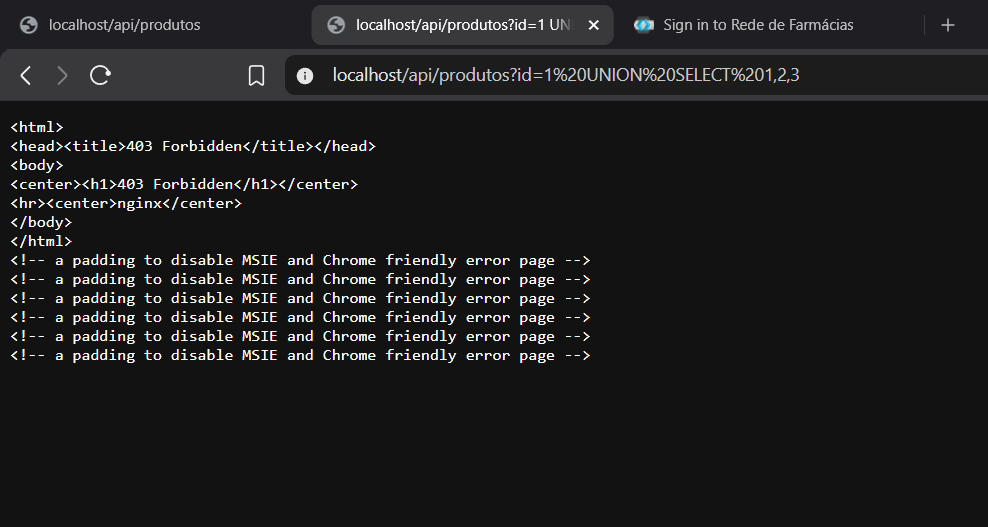
\includegraphics[width=0.82\textwidth]{images/print2_waf_sqli_403.png}
    \caption{Bloqueio perimetral de injeção de SQL retornando código HTTP 403 Forbidden.}
    \label{fig:momento2}
\end{figure}

\textbf{Descrição do que está sendo feito:} Teste de segurança ofensiva/defensiva. Disparo de requisição maliciosa simulando SQL Injection (\texttt{UNION SELECT}) via parâmetro GET. O ModSecurity com OWASP CRS na DMZ intercepta o padrão malicioso e rejeita imediatamente a conexão com status \texttt{HTTP 403 Forbidden} antes de qualquer contato com o backend.

\newpage

\subsection{Momento 3: Gestão de Identidade e Acesso (Keycloak IAM e Usuário Obrigatório)}
\textbf{Atividade Trello correspondente:} \textit{Keycloak IAM com MFA (TOTP) / Configuração de Usuários de Menor Privilégio} (Coluna: Concluído).

\begin{figure}[h!]
    \centering
    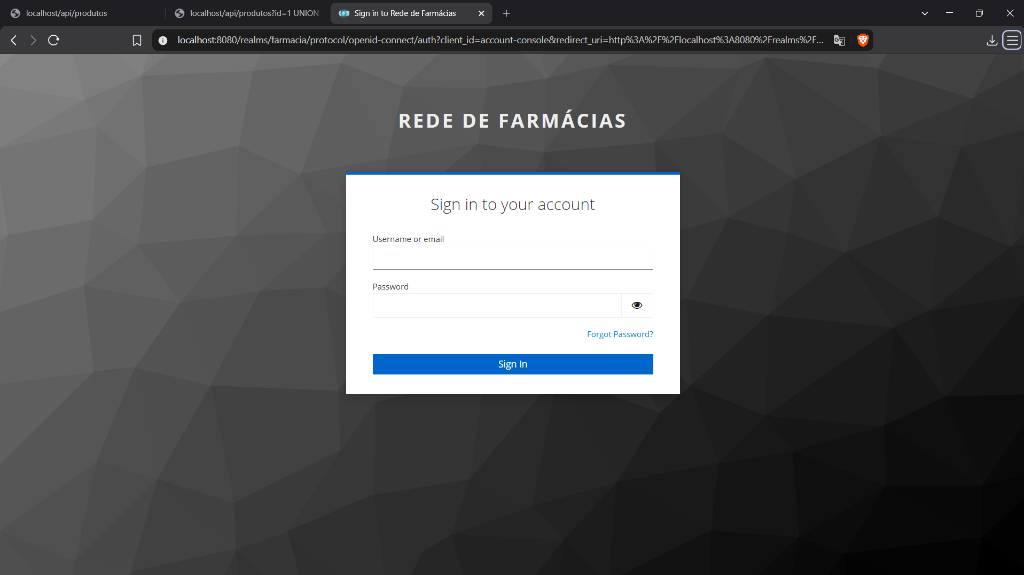
\includegraphics[width=0.85\textwidth]{images/print3_keycloak_iam.png}
    \caption{Tela de login do Keycloak no Realm 'Rede de Farmácias' configurada para o usuário teste.}
    \label{fig:momento3}
\end{figure}

\textbf{Descrição do que está sendo feito:} Configuração do Provedor de Identidade (IAM). A interface de login do Realm \texttt{farmacia} gerencia o acesso seguro e o segundo fator (TOTP). Nela está cadastrado e validado o usuário de menor privilégio obrigatório \texttt{teste@pucparana.com} com a role restrita de \texttt{cliente}.

\end{document}
